\documentclass{article}
\usepackage{tikz}
\usepackage{CJKutf8}
\usepackage{amsmath}
\usepackage{amsthm}
\begin{document}
\begin{CJK}{UTF8}{gbsn}
\newtheorem*{Ex}{习题}
  \begin{Ex}
    设在一个长为$n$的圈外再加一个新的顶点,并且新顶点与圈上每个顶点联结一条边,
    所得到的图称为轮,新加的边称为轮的辐。在有$n$条辐的轮中,给出一个求生成树棵数的公式。
  \end{Ex}

  \begin{proof}[解]

    我们利用c图的生成树棵数的一个递推公式推导出轮的生成树棵数的计算公式。
设$G$为一个图(允许有环和多重边),$e$为$G$的任意一条不为环的边,则$G$的生成树的棵数$\tau (G)$可以计算如下:
\begin{equation}\label{spanning}
\tau(G) = \tau(G-e) + \tau(G \cdot e)  
\end{equation}

其中$G-e$表示从图$G$中去掉边$e$所得到的图。$G \cdot e$表示从图$G$中去掉边$e$并将
$e$的两个端点视为同一个顶点所得到的图,这个过程称为从图$G$中收缩掉边$e$。

下图给出了从一个图$G$中收缩掉一条边的过程。

\begin{center}
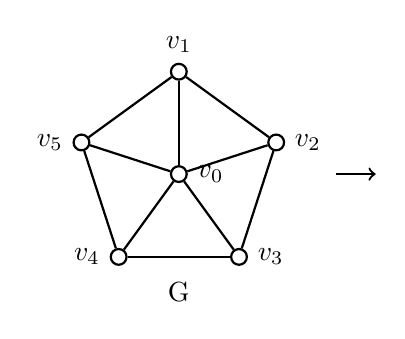
\begin{tikzpicture}[auto,
    specification/.style ={circle, draw, thick, inner sep = 0pt, minimum size=2mm}]
    \node[specification] (A)  [label=0:$v_2$] at (18:1.3cm)  {};
   \node[specification] (B)  [label=90:$v_1$] at (90:1.3cm)  {};
   \node[specification] (C)  [label=180:$v_5$] at (162:1.3cm)  {};
   \node[specification] (D) [label=180:$v_4$] at (234:1.3cm)  {};
   \node[specification] (E)  [label=0:$v_3$] at (306:1.3cm)  {};
   \node[specification] (o)  [label=0:$v_0$] at (0,0)  {};
   \node    at (0,-1.5cm)  {G};

   \draw[->,thick] (2cm,0) to (2.5cm,0);
   
   
   
   \draw[thick] (A) to  (o);
   \draw[thick] (B) to  (o);
   \draw[thick] (C) to  (o);
   \draw[thick] (D) to  (o);
   \draw[thick] (E) to  (o);

   \draw[thick] (A) to  (B);
   \draw[thick] (B) to  (C);
   \draw[thick] (C) to  (D);
   \draw[thick] (D) to  (E);
   \draw[thick] (E) to  (A);


 \end{tikzpicture}
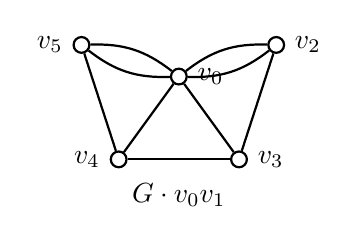
\begin{tikzpicture}[auto,
    specification/.style ={circle, draw, thick, inner sep = 0pt, minimum size=2mm}]
    \node[specification] (A)  [label=0:$v_2$] at (18:1.3cm)  {};
   \node[specification] (C)  [label=180:$v_5$] at (162:1.3cm)  {};
   \node[specification] (D) [label=180:$v_4$] at (234:1.3cm)  {};
   \node[specification] (E)  [label=0:$v_3$] at (306:1.3cm)  {};
   \node[specification] (o)  [label=0:$v_0$] at (0,0)  {};
   \node    at (0,-1.5cm)  {$G\cdot v_0v_1$};

   
   
   \draw[thick] (A) to [bend left = 20]  (o);
   \draw[thick] (A) to [bend right = 20]  (o);

   \draw[thick] (C) to [bend left = 20] (o);
   \draw[thick] (C) to [bend right = 20] (o);
   \draw[thick] (D) to  (o);
   \draw[thick] (E) to  (o);


   \draw[thick] (C) to  (D);
   \draw[thick] (D) to  (E);
   \draw[thick] (E) to  (A);


 \end{tikzpicture}
\end{center}

公式\eqref{spanning}可以推导如下:图$G$中不包含边$e$的生成树的棵数为$\tau(G-e)$,
包含边$e$的生成树的棵数为$\tau(G\cdot e)$,从而图$G$中所有生成树的棵数可以用公式
\eqref{spanning}计算。

有$n$条辐的轮如下图所示:

\begin{center}
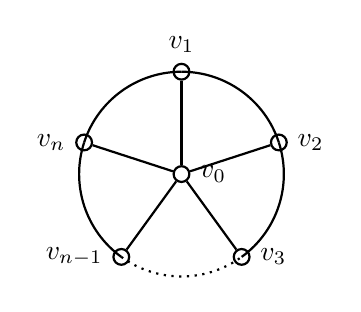
\begin{tikzpicture}[auto,
    specification/.style ={circle, draw, thick, inner sep = 0pt, minimum size=2mm}]
    \node[specification] (A)  [label=0:$v_2$] at (18:1.3cm)  {};
   \node[specification] (B)  [label=90:$v_1$] at (90:1.3cm)  {};
   \node[specification] (C)  [label=180:$v_n$] at (162:1.3cm)  {};
   \node[specification] (D) [label=180:$v_{n-1}$] at (234:1.3cm)  {};
   \node[specification] (E)  [label=0:$v_3$] at (306:1.3cm)  {};
   \node[specification] (o)  [label=0:$v_0$] at (0,0)  {};
   
   
   
   \draw[thick] (A) to  (o);
   \draw[thick] (B) to  (o);
   \draw[thick] (C) to  (o);
   \draw[thick] (D) to  (o);
   \draw[thick] (E) to  (o);

   

   \draw[thick] (18:1.3cm) arc (18:90:1.3cm);
   \draw[thick] (90:1.3cm) arc (90:162:1.3cm);
   \draw[thick] (162:1.3cm) arc (162:234:1.3cm);

   \draw[thick,dotted] (234:1.3cm) arc (234:306:1.3cm);
   \draw[thick] (306:1.3cm) arc (-54:18:1.3cm);
 \end{tikzpicture}
\end{center}

 有$n$条辐的轮中生成树的棵数记为$w_n$,以下应用公式\eqref{spanning}推导出$w_n$的递推关系式如下:

 \begin{equation}
   \begin{cases}
     w_1 &= 1\\
     w_2 &= 5\\
     w_3 &= 16\\
     w_n &= 4w_{n-1} - 4w_{n-2} + w_{n-3} (n \geq 4)
   \end{cases}
 \end{equation}

 为了简洁,在这里,图中生成树的棵数用图本身表示。$w_n$的推导过程如下:
 \begin{equation*}
   w_n = 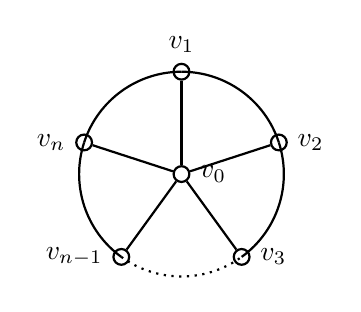
\begin{tikzpicture}[auto,baseline={(current bounding box.center)},
    specification/.style ={circle, draw, thick, inner sep = 0pt, minimum size=2mm}]
    \node[specification] (A)  [label=0:$v_2$] at (18:1.3cm)  {};
   \node[specification] (B)  [label=90:$v_1$] at (90:1.3cm)  {};
   \node[specification] (C)  [label=180:$v_n$] at (162:1.3cm)  {};
   \node[specification] (D) [label=180:$v_{n-1}$] at (234:1.3cm)  {};
   \node[specification] (E)  [label=0:$v_3$] at (306:1.3cm)  {};
   \node[specification] (o)  [label=0:$v_0$] at (0,0)  {};
   
   
   
   \draw[thick] (A) to  (o);
   \draw[thick] (B) to  (o);
   \draw[thick] (C) to  (o);
   \draw[thick] (D) to  (o);
   \draw[thick] (E) to  (o);

   

   \draw[thick] (18:1.3cm) arc (18:90:1.3cm);
   \draw[thick] (90:1.3cm) arc (90:162:1.3cm);
   \draw[thick] (162:1.3cm) arc (162:234:1.3cm);

   \draw[thick,dotted] (234:1.3cm) arc (234:306:1.3cm);
   \draw[thick] (306:1.3cm) arc (-54:18:1.3cm);
 \end{tikzpicture} =
 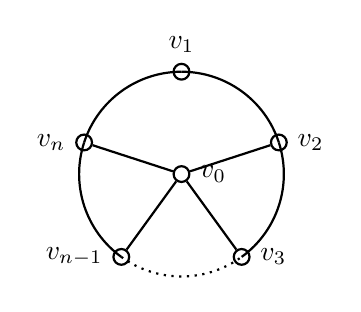
\begin{tikzpicture}[auto,baseline={(current bounding box.center)},
    specification/.style ={circle, draw, thick, inner sep = 0pt, minimum size=2mm}]
    \node[specification] (A)  [label=0:$v_2$] at (18:1.3cm)  {};
   \node[specification] (B)  [label=90:$v_1$] at (90:1.3cm)  {};
   \node[specification] (C)  [label=180:$v_n$] at (162:1.3cm)  {};
   \node[specification] (D) [label=180:$v_{n-1}$] at (234:1.3cm)  {};
   \node[specification] (E)  [label=0:$v_3$] at (306:1.3cm)  {};
   \node[specification] (o)  [label=0:$v_0$] at (0,0)  {};
   
   
   
   
   \draw[thick] (A) to  (o);
   \draw[thick] (C) to  (o);
   \draw[thick] (D) to  (o);
   \draw[thick] (E) to  (o);

   

   \draw[thick] (18:1.3cm) arc (18:90:1.3cm);
   \draw[thick] (90:1.3cm) arc (90:162:1.3cm);
   \draw[thick] (162:1.3cm) arc (162:234:1.3cm);

   \draw[thick,dotted] (234:1.3cm) arc (234:306:1.3cm);
   \draw[thick] (306:1.3cm) arc (-54:18:1.3cm);
 \end{tikzpicture}
 +
 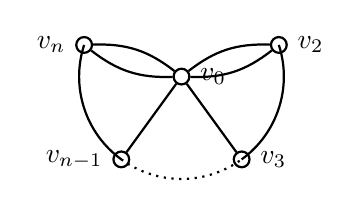
\begin{tikzpicture}[auto,baseline={(current bounding box.center)},
    specification/.style ={circle, draw, thick, inner sep = 0pt, minimum size=2mm}]
    \node[specification] (A)  [label=0:$v_2$] at (18:1.3cm)  {};
   \node[specification] (C)  [label=180:$v_n$] at (162:1.3cm)  {};
   \node[specification] (D) [label=180:$v_{n-1}$] at (234:1.3cm)  {};
   \node[specification] (E)  [label=0:$v_3$] at (306:1.3cm)  {};
   \node[specification] (o)  [label=0:$v_0$] at (0,0)  {};
   
   
   \draw[thick] (A) to [bend left = 20]  (o);
   \draw[thick] (A) to [bend right = 20]  (o);

   \draw[thick] (C) to [bend left = 20] (o);
   \draw[thick] (C) to [bend right = 20] (o);
   
   \draw[thick] (D) to  (o);
   \draw[thick] (E) to  (o);

   

   \draw[thick] (162:1.3cm) arc (162:234:1.3cm);

   \draw[thick,dotted] (234:1.3cm) arc (234:306:1.3cm);
   \draw[thick] (306:1.3cm) arc (-54:18:1.3cm);
 \end{tikzpicture}
 \end{equation*}

 其中
 
\begin{align*}
 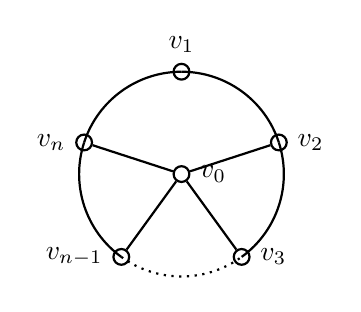
\begin{tikzpicture}[auto,baseline={(current bounding box.center)},
    specification/.style ={circle, draw, thick, inner sep = 0pt, minimum size=2mm}]
    \node[specification] (A)  [label=0:$v_2$] at (18:1.3cm)  {};
   \node[specification] (B)  [label=90:$v_1$] at (90:1.3cm)  {};
   \node[specification] (C)  [label=180:$v_n$] at (162:1.3cm)  {};
   \node[specification] (D) [label=180:$v_{n-1}$] at (234:1.3cm)  {};
   \node[specification] (E)  [label=0:$v_3$] at (306:1.3cm)  {};
   \node[specification] (o)  [label=0:$v_0$] at (0,0)  {};
   \draw[thick] (A) to  (o);
   \draw[thick] (C) to  (o);
   \draw[thick] (D) to  (o);
   \draw[thick] (E) to  (o);
   \draw[thick] (18:1.3cm) arc (18:90:1.3cm);
   \draw[thick] (90:1.3cm) arc (90:162:1.3cm);
   \draw[thick] (162:1.3cm) arc (162:234:1.3cm);
   \draw[thick,dotted] (234:1.3cm) arc (234:306:1.3cm);
   \draw[thick] (306:1.3cm) arc (-54:18:1.3cm);
 \end{tikzpicture}
 &=w_{n-1} + 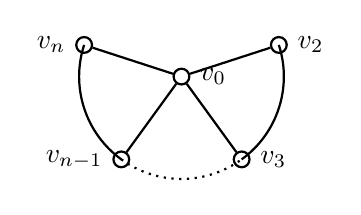
\begin{tikzpicture}[auto,baseline={(current bounding box.center)},
    specification/.style ={circle, draw, thick, inner sep = 0pt, minimum size=2mm}]
    \node[specification] (A)  [label=0:$v_2$] at (18:1.3cm)  {};
   \node[specification] (C)  [label=180:$v_n$] at (162:1.3cm)  {};
   \node[specification] (D) [label=180:$v_{n-1}$] at (234:1.3cm)  {};
   \node[specification] (E)  [label=0:$v_3$] at (306:1.3cm)  {};
   \node[specification] (o)  [label=0:$v_0$] at (0,0)  {};
   \draw[thick] (A) to  (o);
   \draw[thick] (C) to  (o);
   \draw[thick] (D) to  (o);
   \draw[thick] (E) to  (o);
   \draw[thick] (162:1.3cm) arc (162:234:1.3cm);
   \draw[thick,dotted] (234:1.3cm) arc (234:306:1.3cm);
   \draw[thick] (306:1.3cm) arc (-54:18:1.3cm);
 \end{tikzpicture}
\\
  &=2w_{n-1} -
    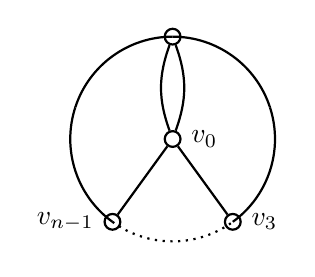
\begin{tikzpicture}[auto,baseline={(current bounding box.center)},
    specification/.style ={circle, draw, thick, inner sep = 0pt, minimum size=2mm}]
   \node[specification] (B)   at (90:1.3cm)  {};
   \node[specification] (D) [label=180:$v_{n-1}$] at (234:1.3cm)  {};
   \node[specification] (E)  [label=0:$v_3$] at (306:1.3cm)  {};
   \node[specification] (o)  [label=0:$v_0$] at (0,0)  {};
   \draw[thick] (B) to [bend left = 20]  (o);
   \draw[thick] (B) to [bend right = 20]  (o);
   \draw[thick] (D) to  (o);
   \draw[thick] (E) to  (o);
   \draw[thick] (18:1.3cm) arc (18:90:1.3cm);
   \draw[thick] (90:1.3cm) arc (90:162:1.3cm);
   \draw[thick] (162:1.3cm) arc (162:234:1.3cm);
   \draw[thick,dotted] (234:1.3cm) arc (234:306:1.3cm);
   \draw[thick] (306:1.3cm) arc (-54:18:1.3cm);
 \end{tikzpicture}
  \\
  &=2w_{n-1} - w_{n-2} -
        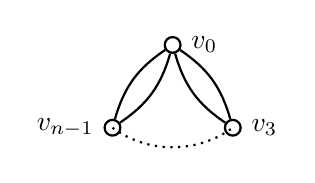
\begin{tikzpicture}[auto,baseline={(current bounding box.center)},
    specification/.style ={circle, draw, thick, inner sep = 0pt, minimum size=2mm}]
   \node[specification] (D) [label=180:$v_{n-1}$] at (234:1.3cm)  {};
   \node[specification] (E)  [label=0:$v_3$] at (306:1.3cm)  {};
   \node[specification] (o)  [label=0:$v_0$] at (0,0)  {};
   \draw[thick] (D) to [bend left = 20]  (o);
   \draw[thick] (D) to [bend right = 20]  (o);
   \draw[thick] (E) to [bend left = 20]  (o);
   \draw[thick] (E) to [bend right = 20]  (o);
   \draw[thick,dotted] (234:1.3cm) arc (234:306:1.3cm);
 \end{tikzpicture}\\
  &=2w_{n-1} - 2w_{n-2} +
        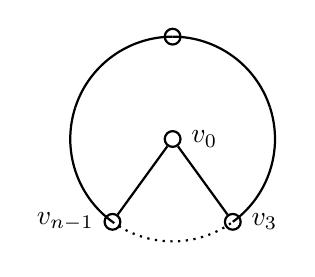
\begin{tikzpicture}[auto,baseline={(current bounding box.center)},
    specification/.style ={circle, draw, thick, inner sep = 0pt, minimum size=2mm}]
   \node[specification] (B)   at (90:1.3cm)  {};
   \node[specification] (D) [label=180:$v_{n-1}$] at (234:1.3cm)  {};
   \node[specification] (E)  [label=0:$v_3$] at (306:1.3cm)  {};
   \node[specification] (o)  [label=0:$v_0$] at (0,0)  {};
   \draw[thick] (D) to  (o);
   \draw[thick] (E) to  (o);
   \draw[thick] (18:1.3cm) arc (18:90:1.3cm);
   \draw[thick] (90:1.3cm) arc (90:162:1.3cm);
   \draw[thick] (162:1.3cm) arc (162:234:1.3cm);
   \draw[thick,dotted] (234:1.3cm) arc (234:306:1.3cm);
   \draw[thick] (306:1.3cm) arc (-54:18:1.3cm);
 \end{tikzpicture}
\end{align*}
\begin{align*}
&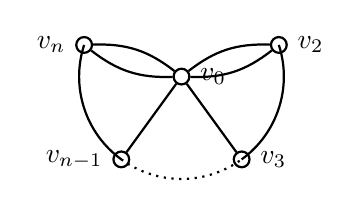
\begin{tikzpicture}[auto,baseline={(current bounding box.center)},
    specification/.style ={circle, draw, thick, inner sep = 0pt, minimum size=2mm}]
    \node[specification] (A)  [label=0:$v_2$] at (18:1.3cm)  {};
   \node[specification] (C)  [label=180:$v_n$] at (162:1.3cm)  {};
   \node[specification] (D) [label=180:$v_{n-1}$] at (234:1.3cm)  {};
   \node[specification] (E)  [label=0:$v_3$] at (306:1.3cm)  {};
   \node[specification] (o)  [label=0:$v_0$] at (0,0)  {};
   \draw[thick] (A) to [bend left = 20]  (o);
   \draw[thick] (A) to [bend right = 20]  (o);
   \draw[thick] (C) to [bend left = 20] (o);
   \draw[thick] (C) to [bend right = 20] (o);
   \draw[thick] (D) to  (o);
   \draw[thick] (E) to  (o);
   \draw[thick] (162:1.3cm) arc (162:234:1.3cm);
   \draw[thick,dotted] (234:1.3cm) arc (234:306:1.3cm);
   \draw[thick] (306:1.3cm) arc (-54:18:1.3cm);
 \end{tikzpicture}\\
  =&
  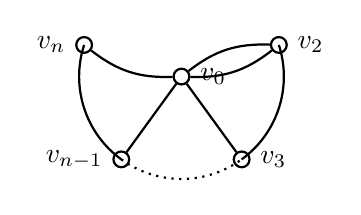
\begin{tikzpicture}[auto,baseline={(current bounding box.center)},
    specification/.style ={circle, draw, thick, inner sep = 0pt, minimum size=2mm}]
    \node[specification] (A)  [label=0:$v_2$] at (18:1.3cm)  {};
   \node[specification] (C)  [label=180:$v_n$] at (162:1.3cm)  {};
   \node[specification] (D) [label=180:$v_{n-1}$] at (234:1.3cm)  {};
   \node[specification] (E)  [label=0:$v_3$] at (306:1.3cm)  {};
   \node[specification] (o)  [label=0:$v_0$] at (0,0)  {};
   \draw[thick] (A) to [bend left = 20]  (o);
   \draw[thick] (A) to [bend right = 20]  (o);
   \draw[thick] (C) to [bend right = 20] (o);
   \draw[thick] (D) to  (o);
   \draw[thick] (E) to  (o);
   \draw[thick] (162:1.3cm) arc (162:234:1.3cm);
   \draw[thick,dotted] (234:1.3cm) arc (234:306:1.3cm);
   \draw[thick] (306:1.3cm) arc (-54:18:1.3cm);
 \end{tikzpicture}+
    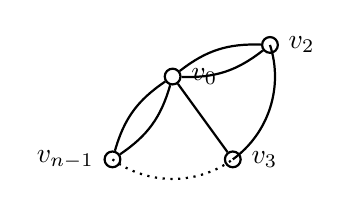
\begin{tikzpicture}[auto,baseline={(current bounding box.center)},
    specification/.style ={circle, draw, thick, inner sep = 0pt, minimum size=2mm}]
    \node[specification] (A)  [label=0:$v_2$] at (18:1.3cm)  {};
   \node[specification] (D) [label=180:$v_{n-1}$] at (234:1.3cm)  {};
   \node[specification] (E)  [label=0:$v_3$] at (306:1.3cm)  {};
   \node[specification] (o)  [label=0:$v_0$] at (0,0)  {};
   \draw[thick] (A) to [bend left = 20]  (o);
   \draw[thick] (A) to [bend right = 20]  (o);
   \draw[thick] (D) to [bend left = 20]  (o);
   \draw[thick] (D) to [bend right = 20]  (o);
   \draw[thick] (E) to  (o);
   \draw[thick,dotted] (234:1.3cm) arc (234:306:1.3cm);
   \draw[thick] (306:1.3cm) arc (-54:18:1.3cm);
 \end{tikzpicture}
  \\
  =&
  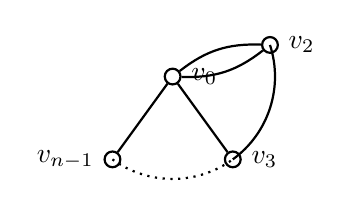
\begin{tikzpicture}[auto,baseline={(current bounding box.center)},
    specification/.style ={circle, draw, thick, inner sep = 0pt, minimum size=2mm}]
    \node[specification] (A)  [label=0:$v_2$] at (18:1.3cm)  {};
   \node[specification] (D) [label=180:$v_{n-1}$] at (234:1.3cm)  {};
   \node[specification] (E)  [label=0:$v_3$] at (306:1.3cm)  {};
   \node[specification] (o)  [label=0:$v_0$] at (0,0)  {};
   \draw[thick] (A) to [bend left = 20]  (o);
   \draw[thick] (A) to [bend right = 20]  (o);
   \draw[thick] (D) to  (o);
   \draw[thick] (E) to  (o);
   \draw[thick,dotted] (234:1.3cm) arc (234:306:1.3cm);
   \draw[thick] (306:1.3cm) arc (-54:18:1.3cm);
 \end{tikzpicture}+
    2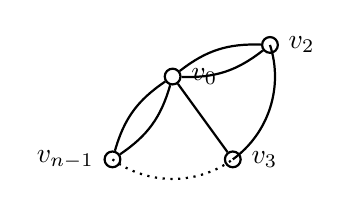
\begin{tikzpicture}[auto,baseline={(current bounding box.center)},
    specification/.style ={circle, draw, thick, inner sep = 0pt, minimum size=2mm}]
    \node[specification] (A)  [label=0:$v_2$] at (18:1.3cm)  {};
   \node[specification] (D) [label=180:$v_{n-1}$] at (234:1.3cm)  {};
   \node[specification] (E)  [label=0:$v_3$] at (306:1.3cm)  {};
   \node[specification] (o)  [label=0:$v_0$] at (0,0)  {};
   \draw[thick] (A) to [bend left = 20]  (o);
   \draw[thick] (A) to [bend right = 20]  (o);
   \draw[thick] (D) to [bend left = 20]  (o);
   \draw[thick] (D) to [bend right = 20]  (o);
   \draw[thick] (E) to  (o);
   \draw[thick,dotted] (234:1.3cm) arc (234:306:1.3cm);
   \draw[thick] (306:1.3cm) arc (-54:18:1.3cm);
 \end{tikzpicture}
  \\
  =&
  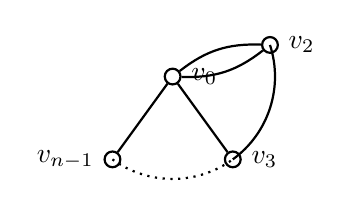
\begin{tikzpicture}[auto,baseline={(current bounding box.center)},
    specification/.style ={circle, draw, thick, inner sep = 0pt, minimum size=2mm}]
    \node[specification] (A)  [label=0:$v_2$] at (18:1.3cm)  {};
   \node[specification] (D) [label=180:$v_{n-1}$] at (234:1.3cm)  {};
   \node[specification] (E)  [label=0:$v_3$] at (306:1.3cm)  {};
   \node[specification] (o)  [label=0:$v_0$] at (0,0)  {};
   \draw[thick] (A) to [bend left = 20]  (o);
   \draw[thick] (A) to [bend right = 20]  (o);
   \draw[thick] (D) to  (o);
   \draw[thick] (E) to  (o);
   \draw[thick,dotted] (234:1.3cm) arc (234:306:1.3cm);
   \draw[thick] (306:1.3cm) arc (-54:18:1.3cm);
 \end{tikzpicture}+
    2(w_{n-1} - 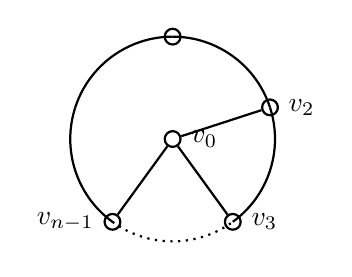
\begin{tikzpicture}[auto,baseline={(current bounding box.center)},
      specification/.style ={circle, draw, thick, inner sep = 0pt, minimum size=2mm}]
   \node[specification] (A)  [label=0:$v_2$] at (18:1.3cm)  {};   
   \node[specification] (B)   at (90:1.3cm)  {};
   \node[specification] (D) [label=180:$v_{n-1}$] at (234:1.3cm)  {};
   \node[specification] (E)  [label=0:$v_3$] at (306:1.3cm)  {};
   \node[specification] (o)  [label=0:$v_0$] at (0,0)  {};
   \draw[thick] (A) to  (o);
   \draw[thick] (D) to  (o);
   \draw[thick] (E) to  (o);
   \draw[thick] (18:1.3cm) arc (18:90:1.3cm);
   \draw[thick] (90:1.3cm) arc (90:162:1.3cm);
   \draw[thick] (162:1.3cm) arc (162:234:1.3cm);
   \draw[thick,dotted] (234:1.3cm) arc (234:306:1.3cm);
   \draw[thick] (306:1.3cm) arc (-54:18:1.3cm);
 \end{tikzpicture})
  \\
    =&
  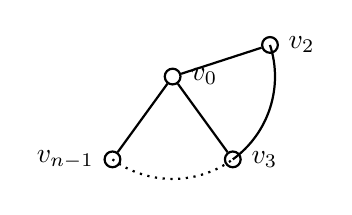
\begin{tikzpicture}[auto,baseline={(current bounding box.center)},
    specification/.style ={circle, draw, thick, inner sep = 0pt, minimum size=2mm}]
    \node[specification] (A)  [label=0:$v_2$] at (18:1.3cm)  {};
   \node[specification] (D) [label=180:$v_{n-1}$] at (234:1.3cm)  {};
   \node[specification] (E)  [label=0:$v_3$] at (306:1.3cm)  {};
   \node[specification] (o)  [label=0:$v_0$] at (0,0)  {};
   \draw[thick] (A) to   (o);
   \draw[thick] (D) to  (o);
   \draw[thick] (E) to  (o);
   \draw[thick,dotted] (234:1.3cm) arc (234:306:1.3cm);
   \draw[thick] (306:1.3cm) arc (-54:18:1.3cm);
 \end{tikzpicture}+
  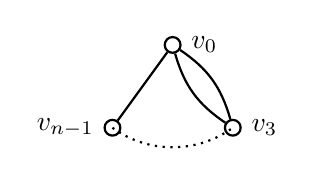
\begin{tikzpicture}[auto,baseline={(current bounding box.center)},
    specification/.style ={circle, draw, thick, inner sep = 0pt, minimum size=2mm}]
   \node[specification] (D) [label=180:$v_{n-1}$] at (234:1.3cm)  {};
   \node[specification] (E)  [label=0:$v_3$] at (306:1.3cm)  {};
   \node[specification] (o)  [label=0:$v_0$] at (0,0)  {};
   \draw[thick] (E) to [bend left = 20]  (o);
   \draw[thick] (E) to [bend right = 20]  (o);
   \draw[thick] (D) to  (o);
   \draw[thick,dotted] (234:1.3cm) arc (234:306:1.3cm);
 \end{tikzpicture}
  \\
  +& 2w_{n-1} -2(  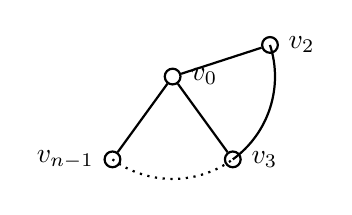
\begin{tikzpicture}[auto,baseline={(current bounding box.center)},
    specification/.style ={circle, draw, thick, inner sep = 0pt, minimum size=2mm}]
    \node[specification] (A)  [label=0:$v_2$] at (18:1.3cm)  {};
   \node[specification] (D) [label=180:$v_{n-1}$] at (234:1.3cm)  {};
   \node[specification] (E)  [label=0:$v_3$] at (306:1.3cm)  {};
   \node[specification] (o)  [label=0:$v_0$] at (0,0)  {};
   \draw[thick] (A) to   (o);
   \draw[thick] (D) to  (o);
   \draw[thick] (E) to  (o);
   \draw[thick,dotted] (234:1.3cm) arc (234:306:1.3cm);
   \draw[thick] (306:1.3cm) arc (-54:18:1.3cm);
 \end{tikzpicture}+w_{n-2}
  )\\
  =&2w_{n-1} - 2w_{n-2} -
  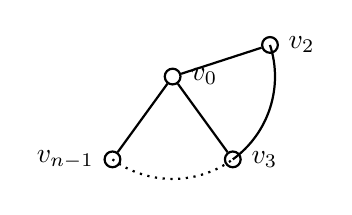
\begin{tikzpicture}[auto,baseline={(current bounding box.center)},
    specification/.style ={circle, draw, thick, inner sep = 0pt, minimum size=2mm}]
    \node[specification] (A)  [label=0:$v_2$] at (18:1.3cm)  {};
   \node[specification] (D) [label=180:$v_{n-1}$] at (234:1.3cm)  {};
   \node[specification] (E)  [label=0:$v_3$] at (306:1.3cm)  {};
   \node[specification] (o)  [label=0:$v_0$] at (0,0)  {};
   \draw[thick] (A) to   (o);
   \draw[thick] (D) to  (o);
   \draw[thick] (E) to  (o);
   \draw[thick,dotted] (234:1.3cm) arc (234:306:1.3cm);
   \draw[thick] (306:1.3cm) arc (-54:18:1.3cm);
 \end{tikzpicture}+
  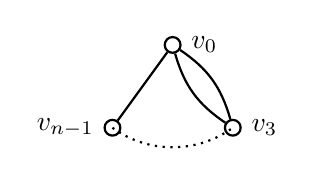
\begin{tikzpicture}[auto,baseline={(current bounding box.center)},
    specification/.style ={circle, draw, thick, inner sep = 0pt, minimum size=2mm}]
   \node[specification] (D) [label=180:$v_{n-1}$] at (234:1.3cm)  {};
   \node[specification] (E)  [label=0:$v_3$] at (306:1.3cm)  {};
   \node[specification] (o)  [label=0:$v_0$] at (0,0)  {};
   \draw[thick] (E) to [bend left = 20]  (o);
   \draw[thick] (E) to [bend right = 20]  (o);
   \draw[thick] (D) to  (o);
   \draw[thick,dotted] (234:1.3cm) arc (234:306:1.3cm);
 \end{tikzpicture}\\
  =&2w_{n-1} - 2w_{n-2} -
  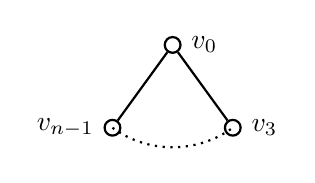
\begin{tikzpicture}[auto,baseline={(current bounding box.center)},
    specification/.style ={circle, draw, thick, inner sep = 0pt, minimum size=2mm}]
   \node[specification] (D) [label=180:$v_{n-1}$] at (234:1.3cm)  {};
   \node[specification] (E)  [label=0:$v_3$] at (306:1.3cm)  {};
   \node[specification] (o)  [label=0:$v_0$] at (0,0)  {};
   \draw[thick] (E) to  (o);
   \draw[thick] (D) to  (o);
   \draw[thick,dotted] (234:1.3cm) arc (234:306:1.3cm);
 \end{tikzpicture}\\
\end{align*}
于是
\begin{align*}
  w_n&=(2w_{n-1} - 2w_{n-2} +
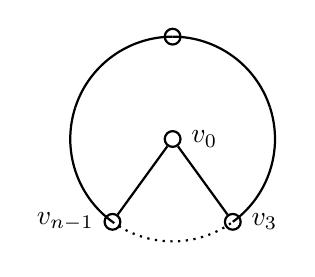
\begin{tikzpicture}[auto,baseline={(current bounding box.center)},
    specification/.style ={circle, draw, thick, inner sep = 0pt, minimum size=2mm}]
   \node[specification] (B)   at (90:1.3cm)  {};
   \node[specification] (D) [label=180:$v_{n-1}$] at (234:1.3cm)  {};
   \node[specification] (E)  [label=0:$v_3$] at (306:1.3cm)  {};
   \node[specification] (o)  [label=0:$v_0$] at (0,0)  {};
   \draw[thick] (D) to  (o);
   \draw[thick] (E) to  (o);
   \draw[thick] (18:1.3cm) arc (18:90:1.3cm);
   \draw[thick] (90:1.3cm) arc (90:162:1.3cm);
   \draw[thick] (162:1.3cm) arc (162:234:1.3cm);
   \draw[thick,dotted] (234:1.3cm) arc (234:306:1.3cm);
   \draw[thick] (306:1.3cm) arc (-54:18:1.3cm);
 \end{tikzpicture})\\
  +&(2w_{n-1} - 2w_{n-2} -
  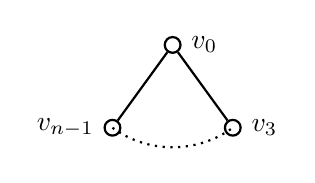
\begin{tikzpicture}[auto,baseline={(current bounding box.center)},
    specification/.style ={circle, draw, thick, inner sep = 0pt, minimum size=2mm}]
   \node[specification] (D) [label=180:$v_{n-1}$] at (234:1.3cm)  {};
   \node[specification] (E)  [label=0:$v_3$] at (306:1.3cm)  {};
   \node[specification] (o)  [label=0:$v_0$] at (0,0)  {};
   \draw[thick] (E) to  (o);
   \draw[thick] (D) to  (o);
   \draw[thick,dotted] (234:1.3cm) arc (234:306:1.3cm);
 \end{tikzpicture})\\
  =&4w_{n-1} - 4w_{n-2} + 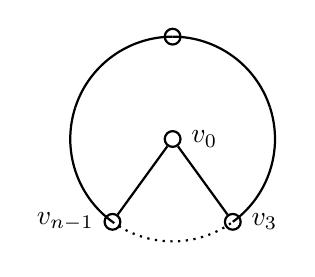
\begin{tikzpicture}[auto,baseline={(current bounding box.center)},
    specification/.style ={circle, draw, thick, inner sep = 0pt, minimum size=2mm}]
   \node[specification] (B)   at (90:1.3cm)  {};
   \node[specification] (D) [label=180:$v_{n-1}$] at (234:1.3cm)  {};
   \node[specification] (E)  [label=0:$v_3$] at (306:1.3cm)  {};
   \node[specification] (o)  [label=0:$v_0$] at (0,0)  {};
   \draw[thick] (D) to  (o);
   \draw[thick] (E) to  (o);
   \draw[thick] (18:1.3cm) arc (18:90:1.3cm);
   \draw[thick] (90:1.3cm) arc (90:162:1.3cm);
   \draw[thick] (162:1.3cm) arc (162:234:1.3cm);
   \draw[thick,dotted] (234:1.3cm) arc (234:306:1.3cm);
   \draw[thick] (306:1.3cm) arc (-54:18:1.3cm);
 \end{tikzpicture}-
  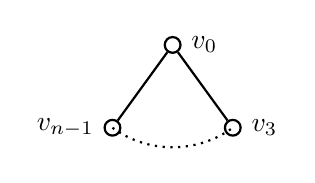
\begin{tikzpicture}[auto,baseline={(current bounding box.center)},
    specification/.style ={circle, draw, thick, inner sep = 0pt, minimum size=2mm}]
   \node[specification] (D) [label=180:$v_{n-1}$] at (234:1.3cm)  {};
   \node[specification] (E)  [label=0:$v_3$] at (306:1.3cm)  {};
   \node[specification] (o)  [label=0:$v_0$] at (0,0)  {};
   \draw[thick] (E) to  (o);
   \draw[thick] (D) to  (o);
   \draw[thick,dotted] (234:1.3cm) arc (234:306:1.3cm);
 \end{tikzpicture}\\
  =&4w_{n-1} - 4w_{n-2} + (w_{n-3} +
    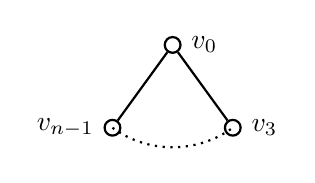
\begin{tikzpicture}[auto,baseline={(current bounding box.center)},
    specification/.style ={circle, draw, thick, inner sep = 0pt, minimum size=2mm}]
   \node[specification] (D) [label=180:$v_{n-1}$] at (234:1.3cm)  {};
   \node[specification] (E)  [label=0:$v_3$] at (306:1.3cm)  {};
   \node[specification] (o)  [label=0:$v_0$] at (0,0)  {};
   \draw[thick] (E) to  (o);
   \draw[thick] (D) to  (o);
   \draw[thick,dotted] (234:1.3cm) arc (234:306:1.3cm);
 \end{tikzpicture}
  )-
    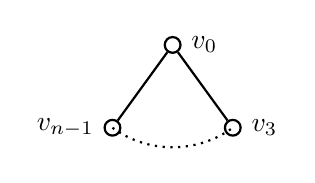
\begin{tikzpicture}[auto,baseline={(current bounding box.center)},
    specification/.style ={circle, draw, thick, inner sep = 0pt, minimum size=2mm}]
   \node[specification] (D) [label=180:$v_{n-1}$] at (234:1.3cm)  {};
   \node[specification] (E)  [label=0:$v_3$] at (306:1.3cm)  {};
   \node[specification] (o)  [label=0:$v_0$] at (0,0)  {};
   \draw[thick] (E) to  (o);
   \draw[thick] (D) to  (o);
   \draw[thick,dotted] (234:1.3cm) arc (234:306:1.3cm);
 \end{tikzpicture}\\
  =&4w_{n-1} - 4w_{n-2} + w_{n-3}
\end{align*}
 $w_n$可以计算如下:
 \begin{equation}\label{result}
   w_n = -2 + (\frac{3-\sqrt{5}}{2})^n + (\frac{3+\sqrt{5}}{2})^n
 \end{equation}
 这是因为设方程
 \begin{equation}\label{characteristic}
   \lambda^3 - 4 \lambda^2 + 4 \lambda - 1 = 0
 \end{equation}
 的任意一个根为$\lambda$,则$w_n = \lambda^n$满足递推关系式:
 \begin{equation}\label{recurrence}
        w_n = 4w_{n-1} - 4w_{n-2} + w_{n-3} (n \geq 4)
 \end{equation}
 方程\eqref{characteristic}可以化为
 \begin{equation*}
   (\lambda -1)(\lambda - \frac{3 - \sqrt{5}}{3})(\lambda - \frac{3 + \sqrt{5}}{3}) = 0   
 \end{equation*}
 其三个根为
 \begin{equation*}
   \begin{cases}
     \lambda_1 &= 1\\
     \lambda_2 &= \frac{3 - \sqrt{5}}{3}\\
     \lambda_3 &= \frac{3 + \sqrt{5}}{3}
   \end{cases}
 \end{equation*}
 则
 \begin{equation}
   \label{eq:recurrence2}
 w_n = C_1  \lambda_1 ^ n + C_2  \lambda_2^n + C_3  \lambda_3^n   
 \end{equation}
 满足递推关系式\eqref{recurrence}。

将$w_1 = 1$,$w_2 = 5$,$w_3 = 16$代入\eqref{eq:recurrence2}得:
 \begin{equation*}
   \begin{cases}
     1 &= C_1  \lambda_1 + C_2  \lambda_2 + C_3  \lambda_3\\
     5 &= C_1  \lambda_1 ^ 2 + C_2  \lambda_2^2 + C_3  \lambda_3^2\\
     16 &= C_1  \lambda_1 ^ 3 + C_2  \lambda_2^3 + C_3  \lambda_3^3
   \end{cases}
 \end{equation*}
解得$C_1=-2,C_2=1,C_3=1$,代入\eqref{eq:recurrence2}便可得\eqref{result}。
% \begin{equation×}
%   2
%   (\lambda -1)(\lambda - \frac{3 + \sqrt{5}}{3})(\lambda - \frac{3 - \sqrt{5}}{3}) = 0
% \end{equation×}
\end{proof}
\end{CJK}
\end{document}


%%% Local Variables:
%%% mode: latex
%%% TeX-master: t
%%% End:
